\chapter*{Fiche pratique}

\addcontentsline{toc}{chapter}{Fiche pratique}

\section{Déroulement :}\\

\begin{itemize}\\
	\item Présentation succinte de la carte Arduino et des éléments de base du kit (BreakBoard, fils d'interconnexion, LEDs, capteurs,...)\\
\begin{figure}[H]
	\begin{center}
		\makebox[\textwidth]{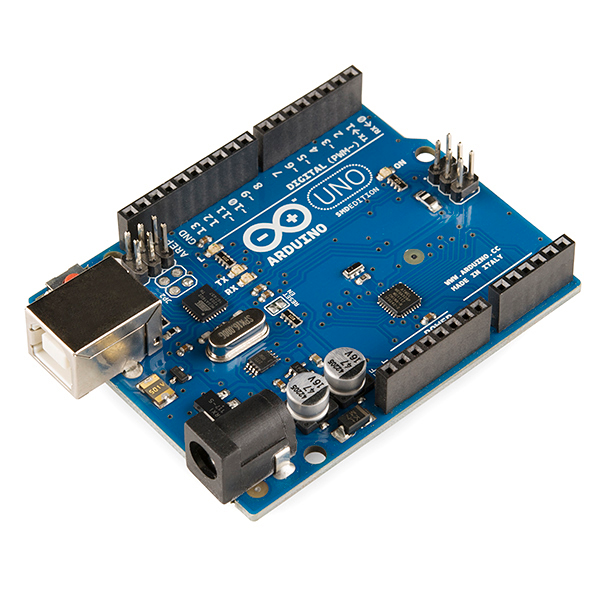
\includegraphics[width=.2\paperwidth]{images/arduino.png}}
	\end{center}
	\caption{ \textit{Une carte Arduino Uno}}
\end{figure}\\

	\item Installation du logiciel Arduino
	\item Découverte du logiciel et des bases de la programmation Arduino
	\item Mise en pratique
	\item Approfondissement
\end{itemize}\\

\section{Mise en pratique : Réalisation d'un feu tricolore}\\

\subsection{Objectifs}\\
\begin{enumerate}\\
	\item Monter un circuit sur BreadBoard permettant d'allumer / éteindre les LEDs grâce à l'Arduino
	\\
	\item Réaliser un petit programme reproduisant le comportement d'un feu tricolore
	\\
\end{enumerate}\\

\begin{figure}[H]
	\begin{center}
		\makebox[\textwidth]{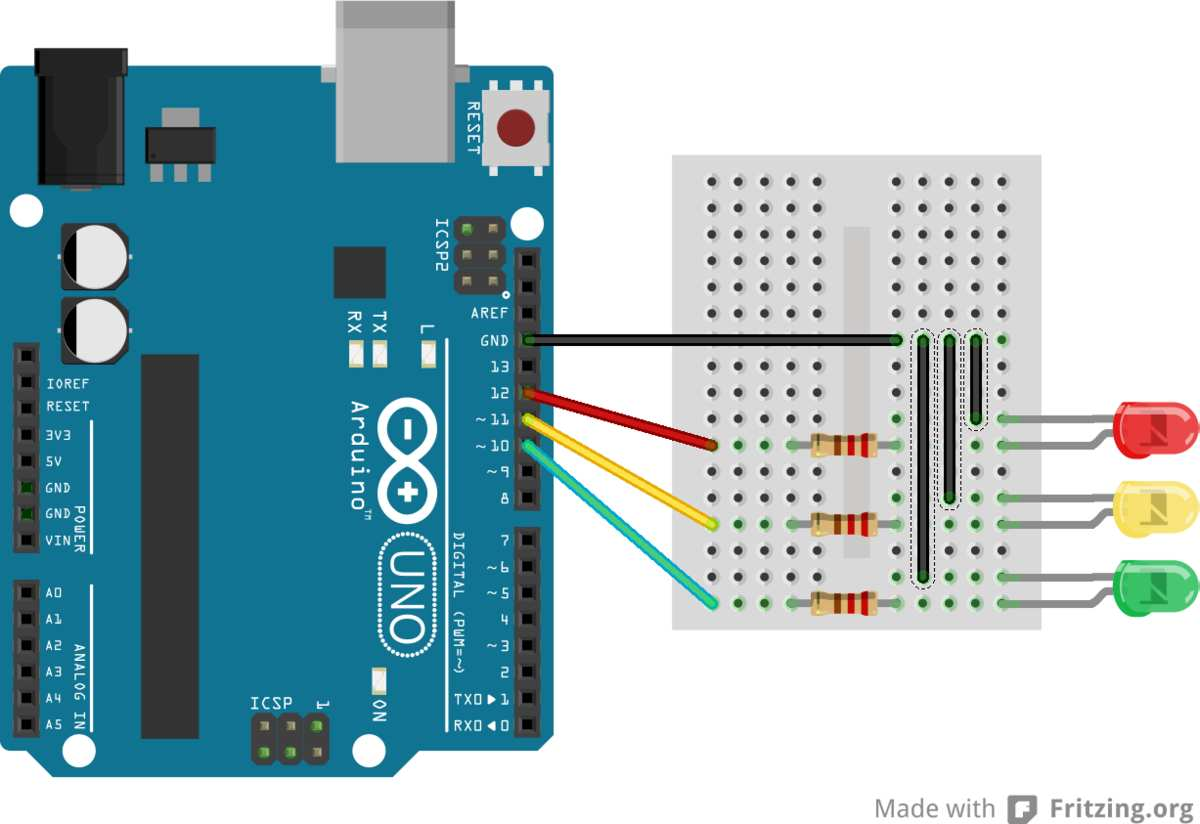
\includegraphics[width=.3\paperwidth]{images/montage1.png}}
	\end{center}
	\caption{ \textit{ Schéma de montage de l'Atelier 1}}
\end{figure}\\

\subsection{Approfondissement}\\

\begin{itemize}\\
	\item Réaliser un petit programme permettant d'utiliser le montage précédent pour compter en binaire.
\end{itemize}\\




